\documentclass[conference]{IEEEtran}
\usepackage{graphicx} % Required for inserting images
\usepackage{epstopdf}
\usepackage{float}
\usepackage{verbatim}
\usepackage{array}
\usepackage{authblk}
% \usepackage{IEEEtrantools}
\usepackage[
    backend=biber,
    style=ieee,
  ]{biblatex}
\addbibresource{additional.bib}  % Additional papers (those not found in SLR)
\usepackage{svg}

\usepackage{xcolor}
\usepackage{longtable}

\begin{document}

\title{Performance Analysis of Cache Size and Set-Associativity Using gem5}

\author[1]{Clayton Asada}
\author[2]{Joseph Chorbajian}
\author[3]{Ilmaan Zia}

\affil[1,2,3]{Computer Engineering and Computer Science, California State University Long Beach}

\date{February 2023}



\maketitle



\begin{abstract}
% TODO: Maybe include most prominent results/analyses in abstract?

\emph{Keywords - } Cache, Size, Associativity, Replacement Policy, gem5, Simulation, Configuration, Miss rate
\end{abstract}

% THIS IS LEFT HERE AS AN EXAMPLE/TEMPLATE FOR INCLUDING PICTURES
% \begin{figure}[H]
%     \centering
%     \includegraphics[width=0.45\textwidth]{images/EmpC1-Training}
%     \caption{Amount of training provided}
%     \label{fig:EmpC1-Training}
% \end{figure}

\section{Introduction}

Cache performance is critical to the performance and efficiency of modern computer systems. As processors have become increasingly fast, the memory and storage hierarchy have struggled to keep up, leading to a performance gap between processors and memory systems. Caches are small, fast memories that sit between the processor and main memory to help bridge this performance gap and supply the processor with data and instructions quickly\cite{hennessy_computer_2012}.

The design of caches involves navigating multiple trade-offs between cache size, associativity, block size, and replacement policies in order to achieve optimal performance for a given workload. Larger cache sizes can store more data, reducing the number of slow accesses to main memory, but have other trade-offs such as having higher access latencies and consuming more power. Associativity refers to the number of locations in the cache that can store a given memory block. Higher associativity reduces conflict misses that occur when two memory blocks map to the same cache location, exchanging for additional hardware cost. Block size determines how much data is brought into the cache at once on a cache miss. Larger block sizes can improve spatial locality and reduce miss rates, but they also bring in more unused data, wasting cache space. Replacement policies determine which cache line is evicted when the cache is full and a new memory block needs to be brought in. More effective replacement policies can improve cache miss rate by reducing the number of useful cache lines evicted\cite{hennessy_computer_2012}.

Simulation tools, like gem5\cite{10.1145/2024716.2024718} and SimpleScalar\cite{10.1145/268806.268810}, are useful for exploring the cache design space and evaluating trade-offs. These tools run simulated workloads and collect various cache metrics across different configurations. This allows designers to find the optimal balance of size, associativity, block size, and replacement policy for a target workload without having to build physical hardware prototypes.

In this paper, we show optimizations of cache miss rates through navigation of these trade-offs. We compare the miss rates on a total of 72 configurations per benchmark by varying cache size, associativity, block size, and replacement policies. Other cache parameters have remained constant. We use three benchmarks from the MiBench benchmark suite, designed for embedded processors. As such, the cache size, block size, and set associativity all match appropriate configurations for embedded processors.

\section{Related Work}

As cache performance is crucial for modern computer systems, computer architecture researchers community has recognized its significance. As a result, cache design has been extensively studied and optimized to improve system performance, with researchers exploring various cache configurations through simulation over decades.

For instance, researchers have explored trade-offs between cache replacement policies. In 2004, Al-Zoubi et. al.\cite{10.1145/986537.986601} evaluated cache replacement policies on the CPU2000 benchmark suite using SimpleScalar and found that LRU and LRU-based policies, specifically pseudo-LRU replacement policies, performed best. More recent studies by Panda et. al.\cite{7806218} shows that modern LRU-based replacement policies outperforming pseudo-LRU using the CPU2006 benchmarks.

Cache size has also been extensively studied. Ma et. al.\cite{5260945} used SimpleScalar to evaluate miss rates across multiple benchmarks in SPEC2000 and found that a larger L1 cache size significantly improves performance when the cache size is small, but gradually decreases as the cache gets bigger. Ullah et. al.\cite{8975563} built on this work by proposing a 2:1 cache rule of thumb, which states that the miss rates of a cache with $n$ cache size and $x$ associativity are equivalent to the miss rates on a configuration with $n/2$ cache size and $2x$ associativity.

While most research on cache configurations and miss rates have been done in SimpleScalar, some research has used gem5. Reas et. al.\cite{10.1109/UKSIM.2010.35} have simulated L2 cache miss rates on m5 (the precursor to gem5) and compared them to miss rates on hardware implementations of their design on the SPLASH-2 benchmark suite.

\section{Motivation}

As stated before, cache performance is a critical factor for any computer system as it plays a significant role in improving system performance and energy efficiency, particularly in memory-intensive workloads. This becomes a greater issue for embedded processors, where speed and energy efficiency have high priority. Therefore, understanding the trade-offs between cache size, associativity, block size, and replacement policies is crucial in the optimization process for processor design.

Furthermore, many simulations of miss rates for various processor configurations use SimpleScalar\cite{10.1145/268806.268810} as their simulator of choice. Original versions of SimpleScalar used its own instruction set architecture derived from MIPS-IV ISA\cite{10.1145/268806.268810} and may not necessarily model real-world processors accurately. While there has been significant research on porting SimpleScalar to different architectures, such as PowerPC, x86, and ARM\cite{10.1145/986537.986601} (with ARM being verified as cycle-accurate\cite{CHUNG2006137}), most research papers on simulating miss rates do not specify the version of SimpleScalar used, the computing environment used, or the instruction set architecture it was ran on.

Therefore, we have developed key questions that our paper hopes to answer:

\begin{enumerate}
  \item What is the best configuration for embedded processors on the selected benchmarks?
  \item Does the 2:1 cache rule of thumb hold for the selected benchmarks?
  \item How does gem5 and SimpleScalar differ on simulated cache miss rates?
\end{enumerate}

Our research aims to contribute to the understanding of cache performance and design by using the gem5 simulator to model various single-core CPU cache configurations. To evaluate the effectiveness of gem5 in modeling cache performance compared to SimpleScalar, we base our configurations on configurations used in Ullah et. al.. In addition, we also aim to explore the impact of replacement policies on cache performance. By comparing the results of our study with those of Ullah et. al., we hope to provide a comprehensive picture of cache performance across different simulators and identify any differences in their respective results.

Our research has the potential to inform cache design and optimization, as well as guide future research in this area. By understanding the impact of cache size, associativity, block size, and replacement policies on performance, we can design more effective caches that improve system performance and energy efficiency. Furthermore, by evaluating the effectiveness of simulation tools such as gem5 and SimpleScalar, we can improve the accuracy and efficiency of cache performance modeling.

\section{Research methodology}
In this research, we use the gem5 simulator to model various single-core CPU cache configurations and evaluate their performance under different workloads. We describe the experimental methodology below.

Hardware and Software Configuration:
We use a Linux-based system for our experiments as that is a base requirement for the gem5 simulator. Additionally the research team purposefully used different types of hardware and operating systems to run the simulations to determine if there were any inconsistencies in the gem5 simulator. Two desktop computers, one operating on Ubuntu 22.04 and the other Debian distro, and a third laptop using WSL were used to run the gem5 simulations. We use gem5 version 20.0.0 for our simulations.

Workloads:
We use a variety of benchmark workloads to evaluate the performance of different cache configurations. The specific benchmarks used in this research are Dijkstra, Sha, and Rijndael from the MiBench benchmark suite.

Cache Configurations:
We evaluate 72 cache configurations of different sizes, different block size, associativity, and replacement policies. As seen in the cache sizes configurations used were 16kB, 32kB, and 64kB. Cache block sizes were configuratble to 32 bytes and 64 bytes. The final configurations that were used for the original research was set associativities of 1, 2, 4, and 8. Additionally the following replacement policies were simulated: Least Recently Used (LRU), Random replacement, and First In First Out (FIFO) replacement policy.

Table \ref{table:configurations} shows the various configurations tested. The three benchmarks come from the MiBench benchmark suite, designed for embedded processors \cite{990739}. LRU, Random, and FIFO are common replacement policies. While there may me better replacement policies conceived, for embedded systems their added complexity is limited.

\begin{table}[H]
  \centering
  \begin{tabular}{| m{1.6cm} | m{.75cm} | m{.75cm} | m{.8cm} | m{2.6cm} |}
      \hline
      \textbf{Benchmarks} & \textbf{Cache Size} & \textbf{Block Size}& \textbf{Set Assoc.}& \textbf{Replacement Policy} \\ \hline
      Dijkstra    &   16kB  &   32    &  1   &    Least Recently Used     \\ \hline
      Sha         &   32kB  &   64    &  2   &    Random                  \\ \hline
      Rijndael    &   64kB  &         &  4   &    First-In First-Out      \\ \hline
                  &         &         &  8   &                            \\ \hline
  \end{tabular}
  \caption{The different configurations tested.}
  \label{table:configurations}
\end{table}

Simulation Setup:
We use gem5's full-system mode to simulate our experiments. In this mode, the entire system, including the CPU, cache, and memory hierarchy, is simulated. We run each workload multiple times to ensure the stability of the results and use a warm-up period to ensure that the cache is populated before we start collecting performance data.

Performance Metrics:
We collect several performance metrics, including execution time, instruction throughput, and cache hit rate. We also collect cache miss rate, cache eviction rate, and average memory access latency to provide a more detailed analysis of cache behavior.

In summary, our experimental methodology involves using the gem5 simulator to evaluate various single-core CPU cache configurations under different workloads. We use a range of performance metrics to compare the performance of different configurations and compare our findings with those of other works to determine the significance of our results.

\section{Results}
In this section the results of each simulation, by benchmark, will be review and thoroughly discussed and analyzed. The target benchmarks are Sha, Dijkstra, and Rijndael.

\subsection{Sha Benchmark}
In order to evaluate the performance, we conducted a benchmark test using the SHA (Secure Hash Algorithm).SHA is a family of cryptographic hash functions that are used to generate a fixed-size message digest from input data of any size. The message digest is designed to be unique and non-reversible, which makes it useful for verifying the integrity and authenticity of digital information.There are currently several variants of the SHA algorithm, including SHA-1, SHA-2 (which includes SHA-224, SHA-256, SHA-384, and SHA-512), and SHA-3.

For the observation, we calculated the cache miss rate using the LRU replacement policy, grouping it with block sizes of 32 and 64, and varying the cache sizes of 16kb, 32kb, and 64kb. Fig 1 illustrates the results of our experiments.

\begin{figure}[H]
    \centering
    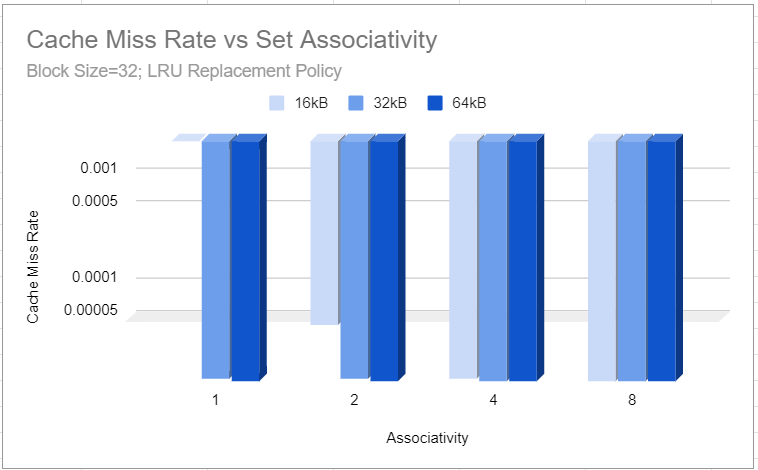
\includegraphics[width=0.45\textwidth]{sha/sha_cache_vs_setAssocBL32.png}
    \caption{The bar chart illustrates the cache miss rates for different cache sizes, including 16KB, 32KB, and 64KB with LRU replacement policy and 32 block size.}
    % \label{fig:EmpC1-Training}
\end{figure}

With a block size of 32 and a cache size of 16kb, and a set associativity of 1, we observed a cache miss rate of 0.002082. However, as the set associativity increased from 2 to 4, we noticed a drop in the cache miss rate. On the other hand, with cache sizes of 32kb and 64kb, the cache miss rate showed less deviation regardless of the set associativity.

\begin{figure}[H]
    \centering
    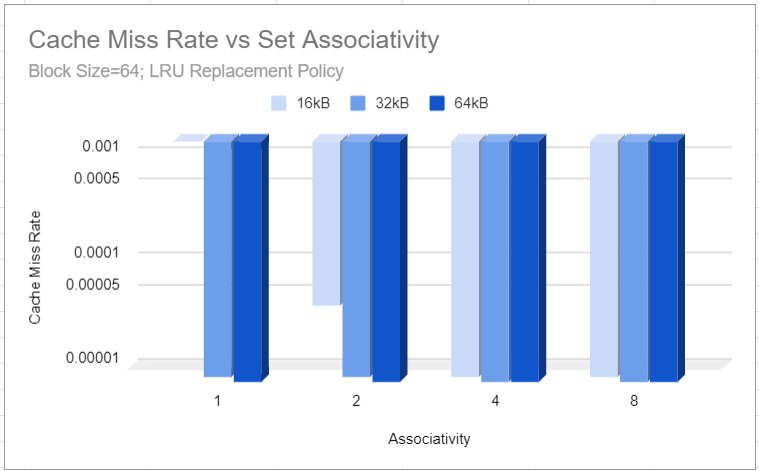
\includegraphics[width=0.45\textwidth]{sha/sha_cache_vs_setAssocBL64.png}
    \caption{The bar chart illustrates the cache miss rates for different cache sizes, including 16KB, 32KB, and 64KB with LRU replacement policy and 64 block size.}
    % \label{fig:EmpC1-Training}
\end{figure}

Figure 2 presents the cache miss rate results with a block size set as 64, a cache size of 16kb, and a set associativity of 1. In this configuration, the cache miss rate was observed to be 0.001342. Interestingly, when comparing the results with block sizes of 32 and 64, we noticed that the cache miss rate with a block size of 64 was nearly half of that with a block size of 32.


\begin{figure}[H]
    \centering
    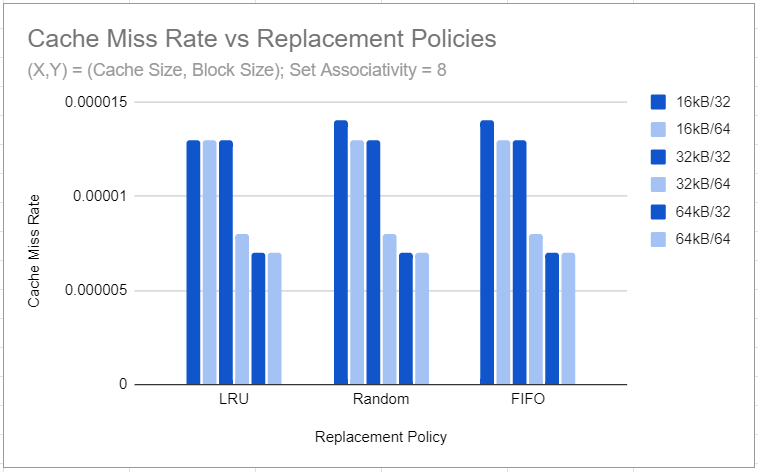
\includegraphics[width=0.45\textwidth]{sha/sha_cache_vs_repl8.png}
    \caption{Cache miss rates with different replacement policies (LRU, Random, and FIFO) with varying the cache sizes and block sizes.}
    % \label{fig:EmpC1-Training}
\end{figure}

Fig3 shows a bar chart indicating that all three replacement policies exhibit certain similarities in their cache miss rates across different variations of cache size and block size.


We observed that the Random and FIFO replacement policies had similar cache miss rates when using a 16kb cache size and a block size of 32. However, the LRU replacement policy had a slightly lower cache miss rate under these conditions. Additionally, we observed a significant drop in cache miss rate for all replacement policies when increasing the block size from 32 to 64 in a 32kb cache size. We also observed that the cache miss rate was lowest when using a 64kb cache size and a block size of 32 or 64, regardless of the replacement policy used. This finding was consistent across all three replacement policies (LRU, Random, and FIFO).


From a total of 72 simulations run on the SHA benchmark with multiple configurations, different results were obtained on each iteration. The biggest simulated cache miss rate was 0.002082, while the smallest was 0.000007.

\begin{figure}[H]
    \centering
    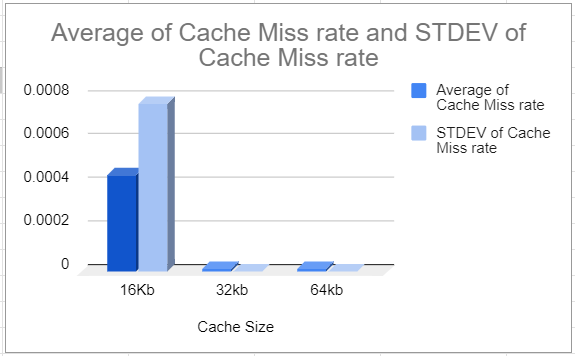
\includegraphics[width=0.45\textwidth]{sha/sha_avg_cachesize.png}
    \caption{The bar chart illustrates the cache miss rates for different cache sizes, including 16KB, 32KB, and 64KB. The x-axis represents the cache size, while the y-axis represents the cache miss rate.}
    % \label{fig:EmpC1-Training}
\end{figure}

The results show that as the cache size increases, the cache miss rate decreases. The cache miss rate for a 16KB cache size was the highest at 0.0004427916667 on average with a standard deviation of 0.0007721100946. However, as the cache size increased to 32KB and 64KB, the cache miss rates decreased significantly to 0.00001034782609 and 0.00001, respectively, with lower standard deviations of 0.000003083809563 and 0.000003064523511. These findings suggest that a larger cache size can significantly improve the performance of the SHA benchmark by reducing the number of cache misses, ultimately leading to faster processing times.

\space


We observed that doubling the block size from 32 to 64 resulted in a significant improvement in performance across different cache sizes, set associativity, and replacement policies. On average, the performance improvement was 41.63%.

The 2:1 rule of thumb, which states that the miss rate of a cache stays the same if the cache size is halved and the block size is doubled, has been widely accepted in computer architecture. However, recent studies have shown that this rule may not hold true for certain workloads. Specifically, in the case of the SHA benchmark, our analysis of 32 tests revealed that the miss rate difference was observed in 18 cases after grouping. This suggests that the 2:1 rule of thumb may not be accurate for this particular workload.


\subsection{Dijkstra Benchmark}

The following section contains the results of simulations using various cache configurations and the Dijkstra benchmark. Each figure allow or paired shows a different aspect of the cache configurations.

\begin{figure}[H]
  \centering
  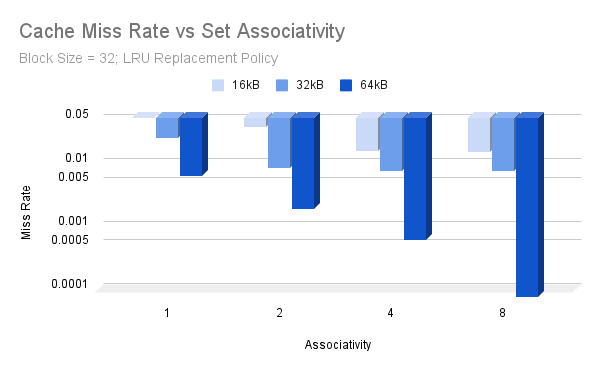
\includegraphics[width=0.45\textwidth]{dijkstraFigures/CacheMissRateVsSetAssociativity32.png}
  \caption{Miss Rate Comparison of Set Associativity with 32 byte Block Size for Dijkstra Benchmark}
  \label{fig:MissRateVsSetAssoc32}
\end{figure}

\begin{figure}[H]
    \centering
    \includegraphics[width=0.45\textwidth]{dijkstraFigures/CacheMissRatevsSetAssociativity64.png}
    \caption{Miss Rate Comparison of Set Associativity with 64 byte Block Size for Dijkstra Benchmark}
    \label{fig:MissRateVsAssoc64}
  \end{figure}
    
The previous two figures depict the miss rate, in log scale, compared to associativity by cache size, with each graph having a fixed replacement policy of LRU and 32 bytes or 64 bytes respectively as the block size. In these charts we can see that associativity has a major impact on miss rate for the Dijkstra benchmark. 8-way set associativity decreased miss rate by orders of magnitude compared to a direct mapped cache. 8-way set associativity for a given cache size, on average, decreased miss rates by 79\%.

When looking at the two charts together, they have only cache replacement policy as a fixed value set to LRU. By comparing like columns, meaning the same cache size, we can compare the effects of cache block size changes for a given set associativity. Looking at the left most columns of each chart, 16kB cache size, we can see that doubling block size does not have nearly the same effect at low associativity, miss reduction of 16\%, as it does with high associativity, reduction of 42\%. Significant difference are seen in performance from both cache size changes and block size. For a 16kB cache, changing the block size from 32 bytes to 64 bytes, is nearly as effective at reducing miss rate as doubling the cache size and maintaining the same block size. This finding did not true from 32kB cache to 64kB cache, but across each configuration, doubling the block size resulted in nearly a 50\% reduction in D-cache miss rate.

Additionally with either graph we can compare miss rates for the 2:1 rule of thumb in cache configurations. This rule states that doubling associativity and halving the cache size should result in equivalent D-cache miss rates. By inspecting column 2 of set associativity 2 groups in Fig. \ref{fig:MissRateVsSetAssoc64}, we find the following cache configuartion, Cache Size: 32kB, Block Size: 64 bytes and Replacement Policy: LRU. Next observe column 1 of group 4-way set associativy in Fig. \ref{fig:MissRateVsSetAssoc64}, the cache configuration is as follows, Cache Size: 16kB, Block Size: 64 bytes and Replacement Policy: LRU. By the rule of thumb we should see that these two columns and configurations resulting in equivalent cache miss rate. This is not what is obversed though. In our simulations using the gem5 simulator and Dijkstra benchmark, here specifically, there is no 2:1 rule of thumb present in any pair of applicable configurations.

Continuing to compare across the graphs, we inspect the D-cache miss rate with respect to block size. By comparing the charts column for column, meaning matching configurations, we are able to fix the cache size, set associativity and replacement policy, to show only the effects of block size on D-cache miss rate. 

While Dijkstra benchmark can be very compute heavy, having to calculate distances for many pairs of nodes, it appears that the 100x100 adjacency matrix was still too small test the effectiveness of cache configurations on a 64kB cache. The minute miss rate shown ing the above figure indicates that a significant majority of the D-cache misses consist of conpulsory cache misses, and once the data is loaded the cache can hold all of the data throughout execution.


\begin{figure}[H]
  \centering
  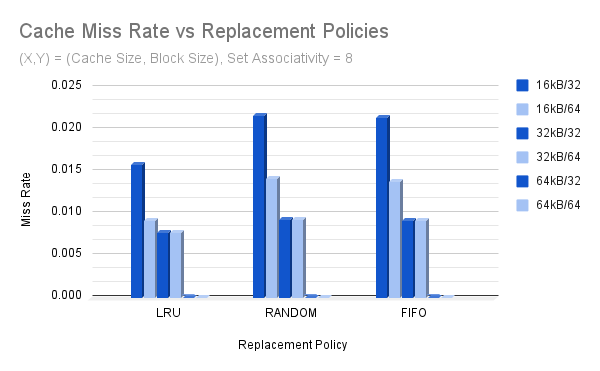
\includegraphics[width=0.45\textwidth]{dijkstraFigures/CacheMissRatevsReplacementPolicies.png}
  \caption{Miss Rate Comparison of Replacement Policies for Dijkstra Benchmark}
  \label{fig:MissRateVsReplPolicy}
\end{figure}

Finally we example replacement policy's effects on cache miss rate. In the figure we have fixed set associativity at 8-way, specifically for the replacement policy to have as many options as possible for choosing a victim block. Here we observe significantly reduced returns as compared to other cache configuration changes. LRU does perform best in almost every case, there were two outlier scenarios of 16kB cache size, block size 32 bytes with 2-way and 4-way associativity having greater performance with Random replacement policy. Overall, First In First Out and Random replacement policies appear equivalent in efficacy. 

While LRU policy does perform best in general across the board implementation of a more complex replacement policy, LRU vs FIFO or Random, may not be worth the effort for hardware architects. Particularly in embedded systems where size, power, and cost are off the utmost importance, these findings indicate that replacement policy would be a good starting point for savings across these three metrics.

\begin{figure}[H]
  \centering
  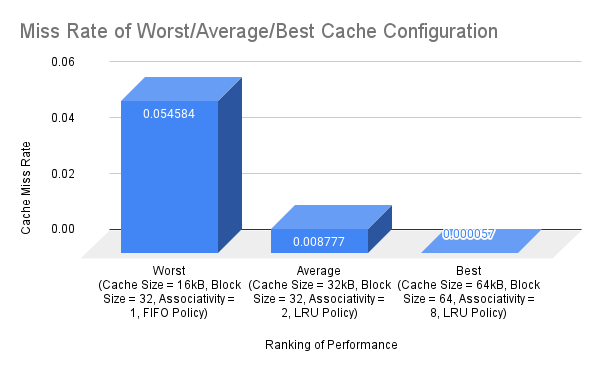
\includegraphics[width=0.45\textwidth]{dijkstraFigures/MissRateofWorstAverageBestCacheConfiguration.png}
  \caption{Miss Rate of Worst, Average, and Best Performing Cache Configurations for Dijkstra Benchmark}
  \label{fig:WorstAvgBest}
\end{figure}

In conclusion of Dijkstra benchmark analysis, the above chart plots the miss rate of the worst, average, and best performing cache configurations. For the Dijkstra benchmark, bigger meant better. Bigger Cache, bigger block size and higher associativity were all guarantees of increased performance and significant reductions in miss rate. Many of the previous charts were unable to effectively depict the miss rate of 64kB cache because its miss rates were so minute.

\subsection{Rijndael Benchmark}

MiBench provides an implementation of Rijndael. While modern desktop CPUs have instructions for Rijndael\cite{gueron2010intel}, they may not be implemented on embedded systems or on systems with small cache configurations. Figure \ref{fig:rijndael-missrate-assoc-32} shows the miss rates on configurations with 16kB, 32kB, and 64kB of cache size; 1, 2, 4, and 8 associativity; and 32 cache size. The configuration with cache size of 16kB and an associativity of 1 shows the highest miss rate at 0.1535. It significantly improves if the cache size or the associativity changes. The miss rates with respect to cache size is monotonically decreasing. That is, a cache size of 16kB with associativity remaining the same will always perform worse than 32kB, and the same with 32kB compared to 64kB. Furthermore, miss rates with respect to associativity also monotonically decreases. The 2:1 cache rule of thumb applies for the configuration of 32kB cache size and 1 associativity compared to the 16kB cache size and 2 associativity, having miss rates 0.0447 and 0.0376, respectively. However, it quickly falls apart with configurations of 64kB cache size and 1 associativity and of 32kB cache size and 2 associativity, having miss rates 0.0383 and 0.0200. The gap continues to increase for larger configurations.

\begin{figure}[H]
    \centering
    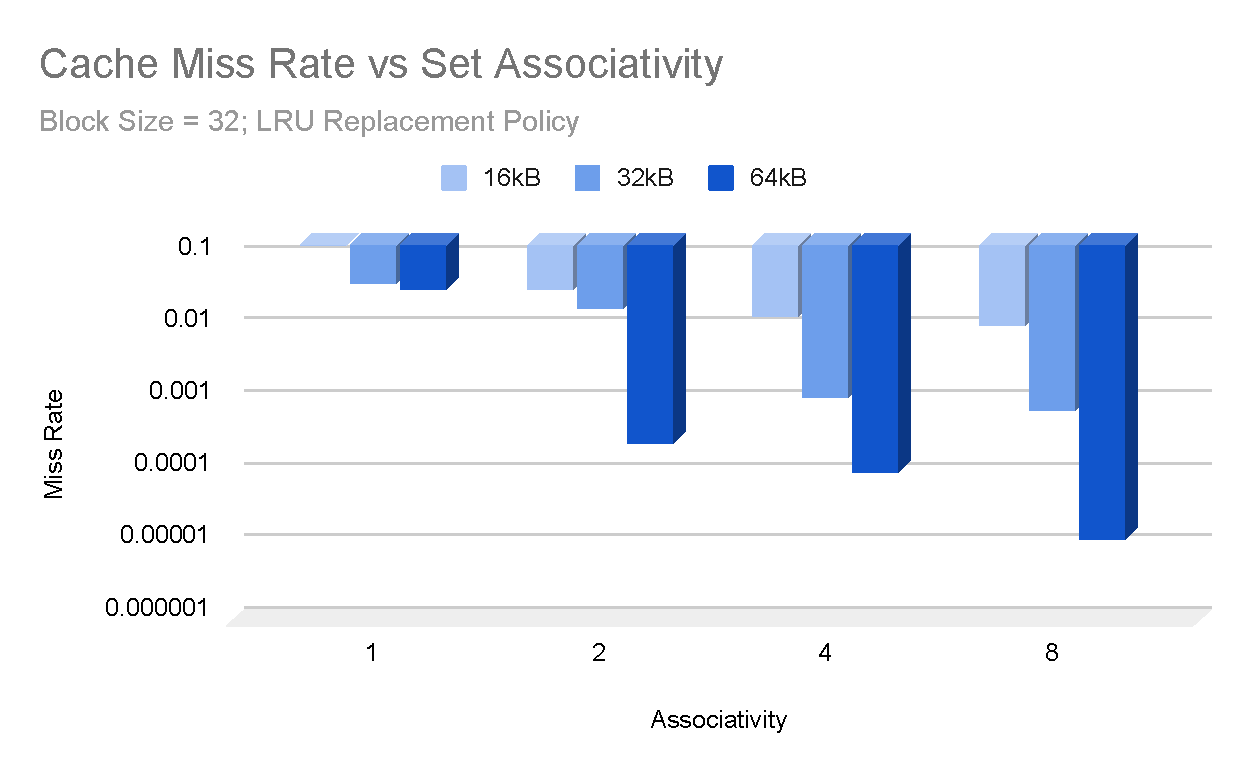
\includegraphics[width=0.45\textwidth]{images/missrate_assoc_32}
    \caption{The miss rate on configurations with different set associativities and cache sizes. The miss rates on the D-cache are on a logarithmic scale to represent the large disparities in the miss rates. Only LRU replacement policy is shown, but the pattern remains the same with other replacement policies (although their extent differs). Smaller values are better.}
    \label{fig:rijndael-missrate-assoc-32}
\end{figure}

Figure \ref{fig:rijndael-missrate-assoc-64} shows the miss rates on configurations similar to that on Figure \ref{fig:rijndael-missrate-assoc-32}, but with 64 block size. The difference in miss rates compared to the 32 block size is less than one percentage point with the exception of a configuration of 16kB of cache size and an associativity of 2, where it has a difference of 1.06\%.

\begin{figure}[H]
  \centering
  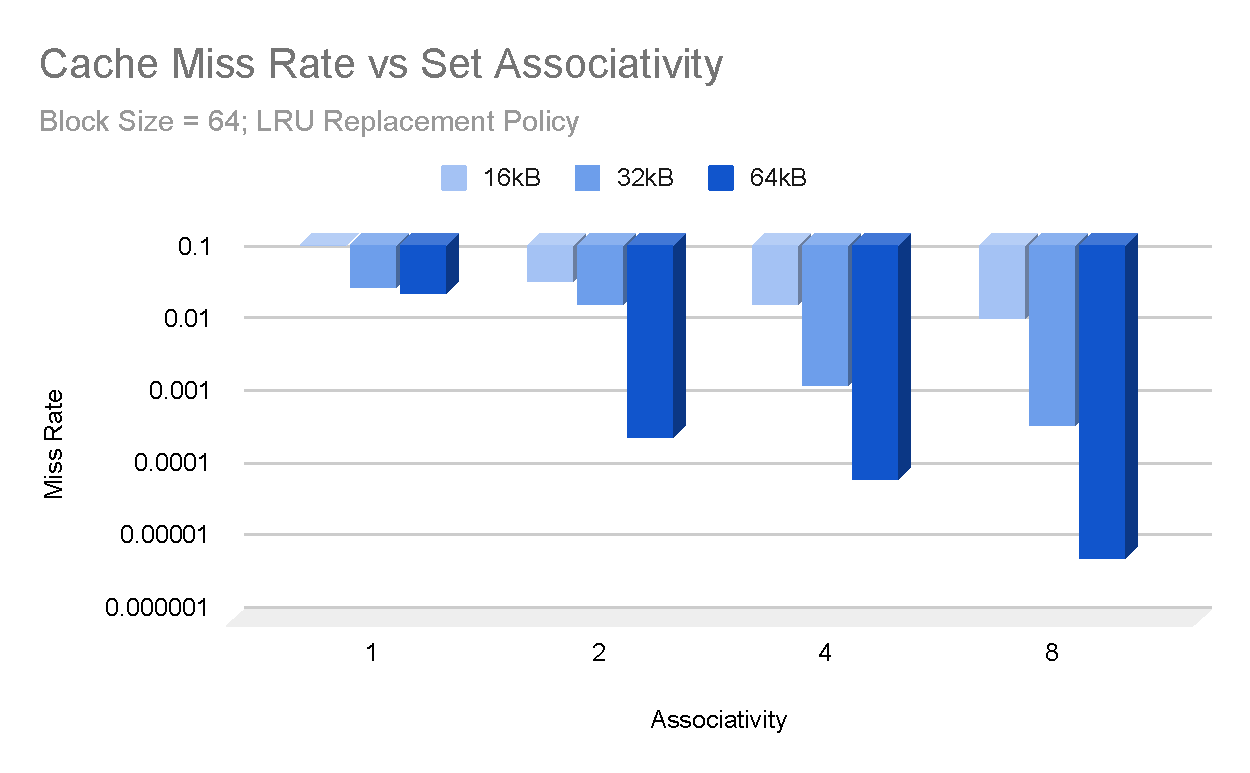
\includegraphics[width=0.45\textwidth]{images/missrate_assoc_64}
  \caption{The D-cache miss rate on configurations with different set associativities and block sizes. Only LRU replacement policy is shown, but the pattern remains the same with other replacement policies (although their extent differs). Log graph, smaller values are better.}
  \label{fig:rijndael-missrate-assoc-64}
\end{figure}

Figure \ref{fig:rijndael-missrate-replacement} shows the miss rates on configurations with varying replacement policies. Similar to other researchers, LRU performs the best out of the three, indicating that it is a good replacement policy and has been simulated correctly. Random has the highest miss rate with a configuration of 16kB of cache size and 64 block size at 0.0278. FIFO outperforms random replacement policy on configurations with 16kB cache size, but random has a lower miss rate for 32kB cache size. For 64kB cache size, they are equal, having 0.000013 and 0.000007 miss rate for 32 and 64 block size, respectively.

\begin{figure}[H]
  \centering
  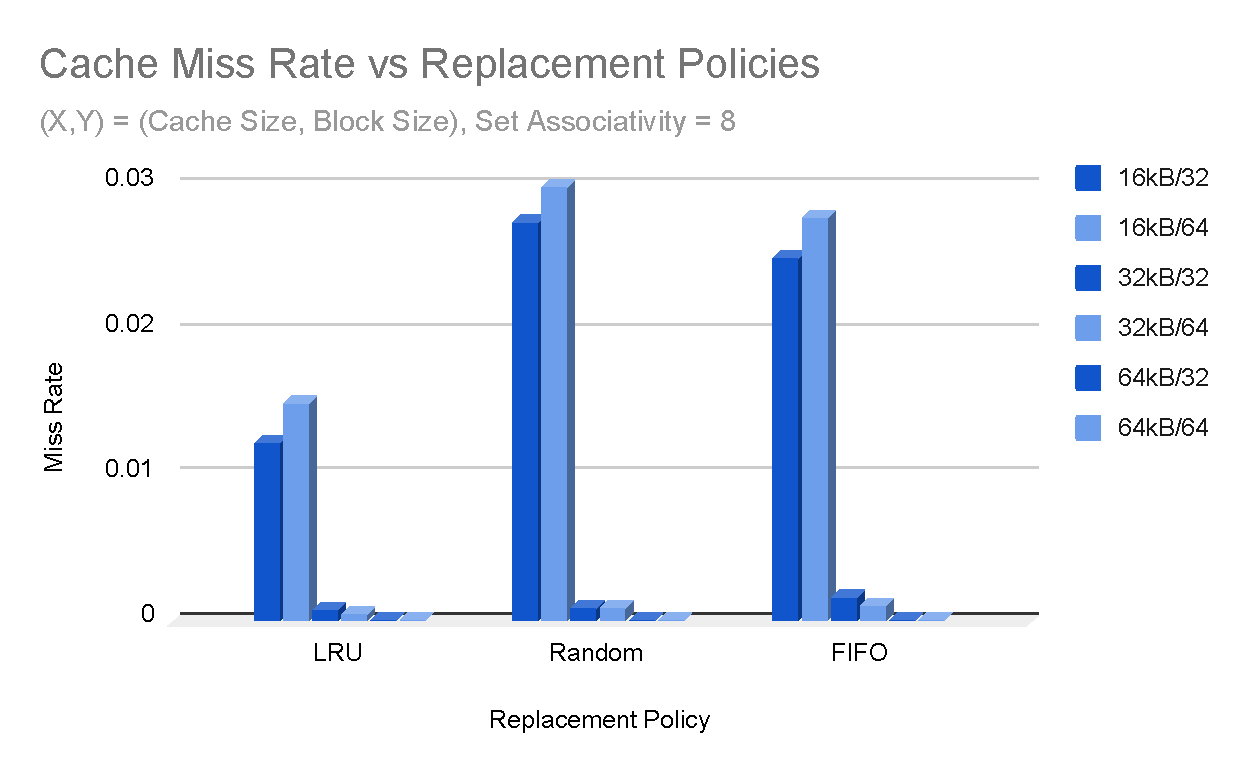
\includegraphics[width=0.45\textwidth]{images/missrate_replacement}
  \caption{The D-cache miss rate on configurations with different replacement policies, cache size, and block size. Only configurations with a set associativity of 8 is shown. Smaller values are better.}
  \label{fig:rijndael-missrate-replacement}
\end{figure}

We explore the pattern of the relative change between block sizes in Figure \ref{fig:rijndael-missrate-percentchange}. Looking solely at the cache size, increasing block size on larger cache size often lowers miss rate. If we break down by associativity, an associativity of 1 always benefits from a larger block size, an associativity of 4 and 8 improve with larger cache sizes. The exception is a configuration with associativity of 2, as that will always benefit from a block size of 32.

\begin{figure}[H]
  \centering
  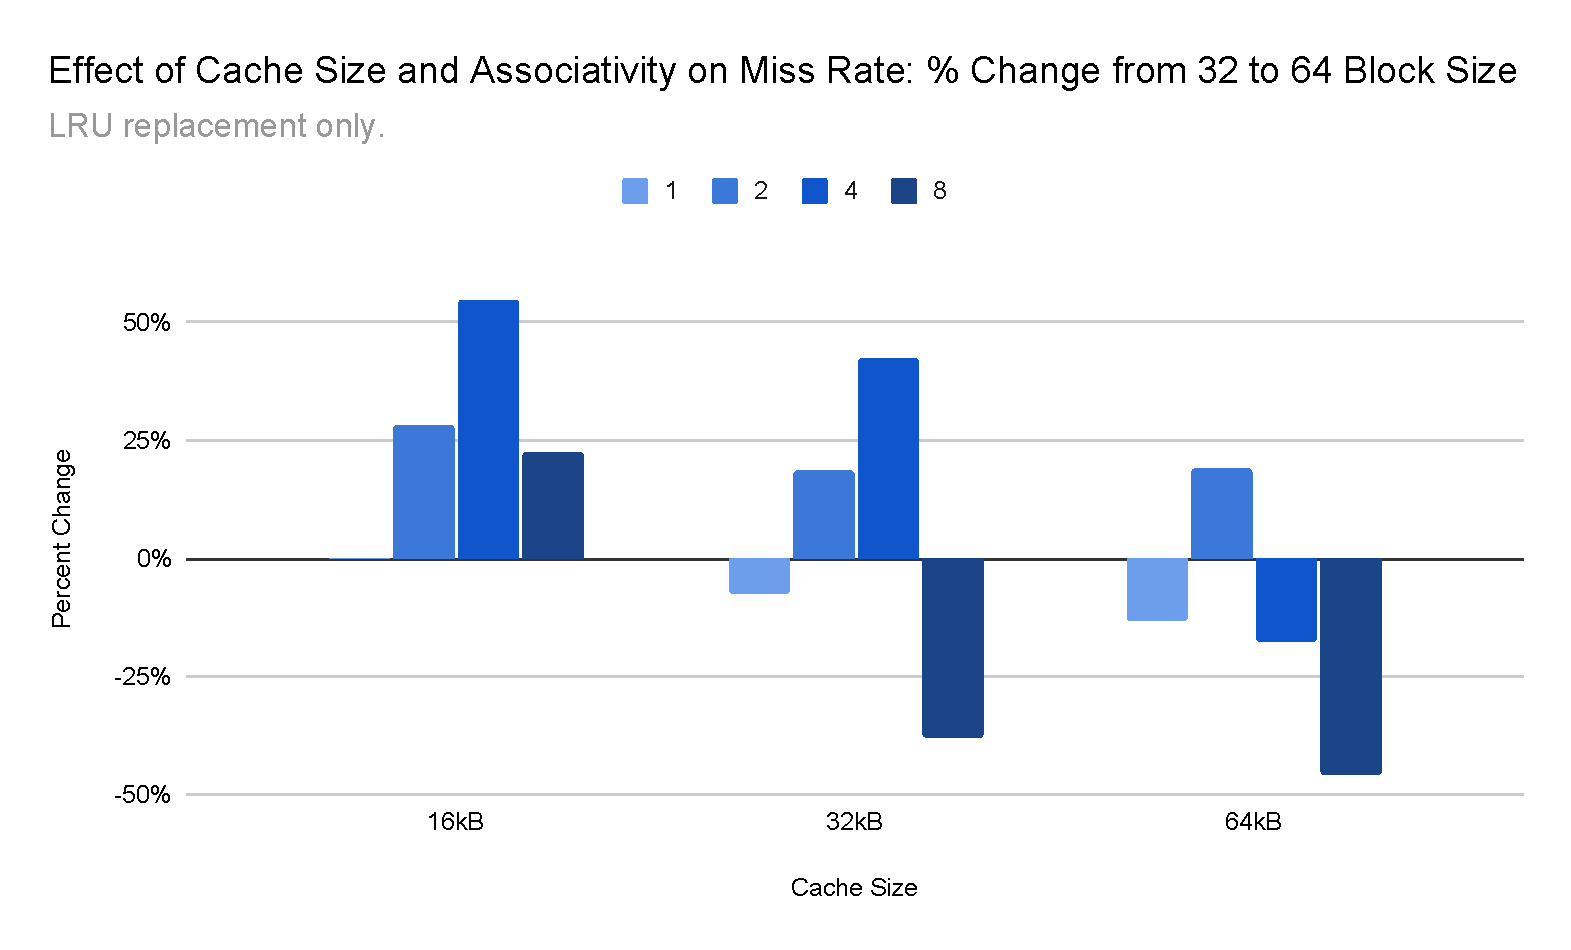
\includegraphics[width=0.45\textwidth]{images/rijndael_missrate_percentchange}
  \caption{The percent change of D-cache miss rate from configurations with 32 vs 64 block size. Only LRU replacement policy is shown, but the pattern remains the same with other replacement policies (although their extent differs).}
  \label{fig:rijndael-missrate-percentchange}
\end{figure}

\section{Discussion}

After running the benchmarks in gem5, we get the best configurations for each benchmark. For SHA, a configuration of 64kB cache size, 64 block size, 8 associativity, and LRU replacement performs the best at a miss rate of 0.000007. For Dijkstra, the same configuration performs the best at a miss rate of 0.000057. Likewise with Rijndael, having a miss rate of 0.000007. Therefore, the configuration with the largest cache size, block size, and associativity with the best replacement policy performs the best, regardless of benchmark. While this specific hardware setup may cost more compared to other configurations, it serves well for the purpose of a generic embedded processor.

The 2:1 cache rule of thumb mostly holds for the SHA benchmark, although the low miss rates may cause it to not hold for even smaller configurations. However, it falls apart for the Dijkstra and Rijndael benchmarks, which are more representative as they have miss rates that differ more on different configurations than SHA. Therefore, we cannot say that this 2:1 cache rule of thumb is an accurate one, even for a rule of thumb.

A discrepancy is formed if we compare results to the results obtained by Ullah et. al.. For example, Ullah et. al. obtains a miss rate of 0.0009 on Rijndael for a configuration of 32kB cache size, 1 associativity, and 32 block size. In our experimental results, the best performing miss rate 0.04346 with FIFO replacement policy. As another example, Ullah et. al. has obtained a miss rate of 0.0011 on the SHA benchmark with 16kB cache size, 2 associativity, and 32 block size. The closest miss rate we have obtained with that same configuration is 0.000044 with FIFO replacement policy.

There may be several possible explanations to these discrepancies. First, they both are simulations and they may have additional error due to any bugs in the simulation software itself. It is difficult to say which simulator is more accurate, so caution is advised for those wishing to reproduce. Furthermore, the environments these simulations are run are most likely different in many regards, including the versions of the benchmark itself. The different instruction set architectures simulated may also play a factor, as most SimpleScalar architectures are RISC-based while x86 is CISC.

\section{Future Work}
The use of gem5 to model various single-core CPU cache configurations provides a powerful tool for evaluating cache performance. Our research has shown that different cache configurations can have a significant impact on performance, and that using simulation tools such as gem5 can provide detailed insights into cache behavior.

There are several directions for future research in this area:

Multi-core CPU Cache Configurations: In this study, we focus on single-core CPU cache configurations. However, multi-core CPUs are becoming increasingly common, and cache design for multi-core CPUs is a complex and challenging area of research. Future studies could use gem5 to model various multi-core CPU cache configurations and evaluate their performance under different workloads.

Machine Learning Techniques: Recent research has explored the use of machine learning techniques to optimize cache performance. These techniques involve using machine learning algorithms to predict cache behavior and optimize cache configurations. Using gem5 to evaluate these techniques can help identify their strengths and weaknesses and guide future research in this area.

Emerging Memory Technologies: Emerging memory technologies, such as phase-change memory (PCM) and resistive random-access memory (RRAM), have the potential to revolutionize cache design. These technologies have different performance characteristics than traditional memory technologies, and designing caches that can take advantage of their unique properties is an area of active research. Future studies could use gem5 to evaluate cache designs that incorporate emerging memory technologies.

Energy-Efficient Caches: Energy efficiency is becoming an increasingly important consideration in cache design. Caches are power-hungry components of the memory hierarchy, and designing energy-efficient caches is essential to reduce power consumption and improve battery life. Future studies could use gem5 to evaluate energy-efficient cache designs, such as cache compression and cache bypassing techniques.

In conclusion, the use of gem5 to model various single-core CPU cache configurations provides a powerful tool for evaluating cache performance. Future research in this area could explore multi-core CPU cache configurations, machine learning techniques, emerging memory technologies, and energy-efficient caches. These studies could provide valuable insights into cache design and help improve the performance and energy efficiency of modern computer systems.

\section{Conclusion}
In this research, we have used the gem5 simulator to model various single-core CPU cache configurations and evaluated their performance using several benchmarks. We compared our results with those of a previous study that used the SimpleScalar simulator to evaluate cache performance. Our research aimed to contribute to the understanding of cache performance and design, as well as evaluate the effectiveness of different simulators in modeling cache behavior.

Our study found that the performance of different cache configurations varied significantly depending on the workload characteristics. We observed that the impact of replacement policies on cache performance was insignificant, with the LRU policy outperforming the FIFO and Random policies in most cases.

Our results differed significantly from those of the previous study, which focused on the impact of cache size and associativity on performance using the SimpleScalar simulator. We found that the performance of cache configurations varied depending on the simulator. Our findings suggest that the gem5 simulator may be more effective in modeling cache behavior of modern CPU's compared to SimpleScalar.

Our research has several implications for cache design and optimization. By understanding the impact of different cache configurations on performance, designers can improve system performance and energy efficiency. Our findings also have implications for the use of simulation tools in cache performance modeling, highlighting the need for careful selection of simulator and benchmark suite.

In conclusion, our research has contributed to the understanding of cache performance and design using the gem5 simulator. Our results highlight the significant differences in cache performance between different simulators and benchmark suites. We hope that our findings will guide future research in cache design and optimization and improve the accuracy and efficiency of cache performance modeling.

\printbibliography
\onecolumn

\appendix
\setcounter{section}{0}
\section{Dijkstra Simulation Data}
    \begin{table}
      \caption{Dijkstra Benchmark}
      \centering
        \begin{tabular}{|m{.75cm} |m{.75cm} |m{.8cm} | m{.75cm} | l | l | l | l | l | l | l |}
          \hline
          \textbf{Cache Size} & \textbf{ Block Size} & \textbf{Set Assoc.} & \textbf{Repl. Policy} & \textbf{Inst. Count} & \textbf{IC hit} & \textbf{IC Missed} & \textbf{IC MissRate} & \textbf{DC hit} & \textbf{DC Missed} & \textbf{DC Miss Rate} \\ \hline
          
          										
16kB&	32&	1&	1&	225882042&	319363400&	63949 &0.0002	 & 53844950	  &3108738	&0.054584 \\ \hline
16kB&	32&	1&	2&	225882042&	319363400&	63949 &0.0002	 & 53844950	  &3108738	&0.054584 \\ \hline
16kB&	32&	1&	3&	225882042&	319363400&	63949 &0.0002	 & 53844950	  &3108738	&0.054584 \\ \hline
16kB&	32&	2&	1&	225882042&	319423331&	4018  &0.000013&	54694862	&2258826	&0.039661 \\ \hline
16kB&	32&	2&	2&	225882042&	319422902&	4447  &0.000014&	54905813	&2047875	&0.035957 \\ \hline
16kB&	32&	2&	3&	225882042&	319423032&	4317  &0.000014&	54607742	&2345946	&0.04119  \\ \hline
16kB&	32&	4&	1&	225882042&	319424560&	2789  &0.000009&	56021761	&931927	  &0.016363 \\ \hline
16kB&	32&	4&	2&	225882042&	319424627&	2722  &0.000009&	55728462	&1225226	&0.021513 \\ \hline
16kB&	32&	4&	3&	225882042&	319424033&	3316  &0.00001	&  55746866 &	1206822	&0.02119  \\ \hline
16kB&	32&	8&	1&	225882042&	319426027&	1322  &0.000004&	56049483	&904205	  &0.015876 \\ \hline
16kB&	32&	8&	2&	225882042&	319425830&	1519  &0.000005&	55715846	&1237842	&0.021734 \\ \hline
16kB&	32&	8&	3&	225882042&	319425977&	1372  &0.000004&	55731617	&1222071	&0.021457 \\ \hline
16kB&	64&	1&	1&	225882042&	319392138&	35211 &0.00011	&  54210849 &	2740582	&0.048121 \\ \hline
16kB&	64&	1&	2&	225882042&	319392138&	35211 &0.00011	&  54210849 &	2740582	&0.048121 \\ \hline
16kB&	64&	1&	3&	225882042&	319392138&	35211 &0.00011	&  54210849 &	2740582	&0.048121 \\ \hline
16kB&	64&	2&	1&	225882042&	319424577&	2772  &0.000009&	55027664	&1923767	&0.033779 \\ \hline
16kB&	64&	2&	2&	225882042&	319424252&	3097  &0.00001	&  55123643 &	1827788	&0.032094 \\ \hline
16kB&	64&	2&	3&	225882042&	319424290&	3059  &0.00001	&  54898513 &	2052918	&0.036047 \\ \hline
16kB&	64&	4&	1&	225882042&	319425030&	2319  &0.000007&	56390810	&560621	  &0.009844 \\ \hline
16kB&	64&	4&	2&	225882042&	319425019&	2330  &0.000007&	56156876	&794555	  &0.013951 \\ \hline
16kB&	64&	4&	3&	225882042&	319424507&	2842  &0.000009&	56181918	&769513	  &0.013512 \\ \hline
16kB&	64&	8&	1&	225882042&	319426555&	794	  &0.000002&	56426880	&524551	  &0.00921  \\ \hline
16kB&	64&	8&	2&	225882042&	319426390&	959	  &0.000003&	56139222	&812209	  &0.014261 \\ \hline
16kB&	64&	8&	3&	225882042&	319426520&	829	  &0.000003&	56161253	&790178	  &0.013875 \\ \hline
32kB&	32&	1&	1&	225882042&	319423518&	3831  &0.000012&	55489194	&1464494	&0.025714 \\ \hline
32kB&	32&	1&	2&	225882042&	319423518&	3831  &0.000012&	55489194	&1464494	&0.025714 \\ \hline
32kB&	32&	1&	3&	225882042&	319423518&	3831  &0.000012&	55489194	&1464494	&0.025714 \\ \hline
32kB&	32&	2&	1&	225882042&	319425809&	1540  &0.000005&	56453802	&499886	  &0.008777 \\ \hline
32kB&	32&	2&	2&	225882042&	319425775&	1574  &0.000005&	56369181	&584507	  &0.010263 \\ \hline
32kB&	32&	2&	3&	225882042&	319425820&	1529  &0.000005&	56368002	&585686	  &0.010284 \\ \hline
32kB&	32&	4&	1&	225882042&	319426035&	1314  &0.000004&	56502425	&451263	  &0.007923 \\ \hline
32kB&	32&	4&	2&	225882042&	319425985&	1364  &	0.000004  &	56402575  &	551113	&0.009677 \\ \hline
32kB&	32&	4&	3&	225882042&	319426025&	1324  &	0.000004  &	56407995  &	545693	&0.009581 \\ \hline
32kB&	32&	8&	1&	225882042&	319426035&	1314  &	0.000004  &	56506962  &	446726	&0.007844 \\ \hline
32kB&	32&	8&	2&	225882042&	319425972&	1377  &	0.000004  &	56422545  &	531143	&0.009326 \\ \hline
32kB&	32&	8&	3&	225882042&	319426026&	1323  &	0.000004  &	56425358  &	528330	&0.009276 \\ \hline
32kB&	64&	1&	1&	225882042&	319424696&	2653  &	0.000008  &	55663535  &	1287896	&0.022614 \\ \hline
32kB&	64&	1&	2&	225882042&	319424696&	2653  &	0.000008  &	55663535  &	1287896	&0.022614 \\ \hline
32kB&	64&	1&	3&	225882042&	319424696&	2653  &	0.000008  &	55663535  &	1287896	&0.022614 \\ \hline
32kB&	64&	2&	1&	225882042&	319426453&	896	  &0.000003	  &56644758	  &306673	  &0.005385 \\ \hline
32kB&	64&	2&	2&	225882042&	319426421&	928	  &0.000003	  &56580462	  &370969	  &0.006514 \\ \hline
32kB&	64&	2&	3&	225882042&	319426470&	879	  &0.000003	  &56585160	  &366271	  &0.006431 \\ \hline
32kB&	64&	4&	1&	225882042&	319426573&	776	  &0.000002	  &56694001	  &257430	  &0.00452 \\ \hline
32kB&	64&	4&	2&	225882042&	319426521&	828	  &0.000003	  &56614011	  &337420	  &0.005925 \\ \hline
32kB&	64&	4&	3&	225882042&	319426561&	788	  &0.000002	  &56619458	  &331973	  &0.005829 \\ \hline
32kB&	32&	8&	1&	225882042&	319426035&	1314  &	0.000004  &	56506962  &	446726	&0.007844 \\ \hline
32kB&	32&	8&	2&	225882042&	319425972&	1377  &	0.000004  &	56422545  &	531143	&0.009326 \\ \hline
32kB&	32&	8&	3&	225882042&	319426026&	1323  &	0.000004  &	56425358  &	528330	&0.009276 \\ \hline
64kB&	32&	1&	1&	225882042&	319425599&	1750  &	0.000005  &	56589626  &	364062	&0.006392 \\ \hline
64kB&	32&	1&	2&	225882042&	319425599&	1750  &	0.000005  &	56589626  &	364062	&0.006392 \\ \hline
64kB&	32&	1&	3&	225882042&	319425599&	1750  &	0.000005  &	56589626  &	364062	&0.006392 \\ \hline
64kB&	32&	2&	1&	225882042&	319425821&	1528  &	0.000005  &	56844976  &	108712	&0.001909 \\ \hline
64kB&	32&	2&	2&	225882042&	319425849&	1500  &	0.000005  &	56812936  &	140752	&0.002471 \\ \hline
64kB&	32&	2&	3&	225882042&	319425848&	1501  &	0.000005  &	56817912  &	135776	&0.002384 \\ \hline
64kB&	32&	4&	1&	225882042&	319426036&	1313  &	0.000004  &	56918063  &	35625	  &0.000626 \\ \hline
64kB&	32&	4&	2&	225882042&	319426034&	1315  &	0.000004  &	56905687  &	48001	  &0.000843 \\ \hline
64kB&	32&	4&	3&	225882042&	319426035&	1314  &	0.000004  &	56903637  &	50051	  &0.000879 \\ \hline
64kB&	32&	8&	1&	225882042&	319426036&	1313  &	0.000004  &	56949333  &	4355	  &0.000076 \\ \hline
64kB&	32&	8&	2&	225882042&	319426035&	1314  &	0.000004  &	56947976  &	5712	  &0.0001 \\ \hline
64kB&	32&	8&	3&	225882042&	319426036&	1313  &	0.000004  &	56947966  &	5722	  &0.0001 \\ \hline
64kB&	64&	1&	1&	225882042&	319426340&	1009  &	0.000003  &	56679489  &	271942	&0.004775 \\ \hline
64kB&	64&	1&	2&	225882042&	319426340&	1009  &	0.000003  &	56679489  &	271942	&0.004775 \\ \hline
64kB&	64&	1&	3&	225882042&	319426340&	1009  &	0.000003  &	56679489  &	271942	&0.004775 \\ \hline
64kB&	64&	2&	1&	225882042&	319426463&	886	  &0.000003	  &56882379	  &69052	  &0.001212 \\ \hline
64kB&	64&	2&	2&	225882042&	319426480&	869	  &0.000003	  &56858757	  &92674	  &0.001627 \\ \hline
64kB&	64&	2&	3&	225882042&	319426492&	857	  &0.000003	  &56863394	  &88037	  &0.001546 \\ \hline
64kB&	64&	4&	1&	225882042&	319426574&	775	  &0.000002	  &56929917	  &21514	  &0.000378 \\ \hline
64kB&	64&	4&	2&	225882042&	319426570&	779	  &0.000002	  &56920955	  &30476	  &0.000535 \\ \hline
64kB&	64&	4&	3&	225882042&	319426573&	776	  &0.000002	  &56919509	  &31922	  &0.000561 \\ \hline
64kB&	64&	8&	1&	225882042&	319426574&	775	  &0.000002	  &56948181	  &3250	    &0.000057 \\ \hline
64kB&	64&	8&	2&	225882042&	319426572&	777	  &0.000002	  &56947025	  &4406	    &0.000077 \\ \hline
64kB&	64&	8&	3&	225882042&	319426574&	775	  &0.000002	  &56946405	  &5026	    &0.000088 \\ \hline
    \end{tabular}
  \end{table}

  \section{Rijndael Simulation Data}
  \begin{table}
    \caption{Rijndael Benchmark. \\ Replacement policy of 1 is LRU, 2 is Random, 3 is FIFO. IC and DC refer to instruction and data cache, respectively.}
    \centering
      \begin{tabular}{|m{.75cm} |m{.75cm} |m{.8cm} | m{.75cm} | l | l | l | l | l | l | l |}
        \hline
        \textbf{Cache Size} & \textbf{ Block Size} & \textbf{Set Assoc.} & \textbf{Repl. Policy} & \textbf{Inst. Count} & \textbf{IC hit} & \textbf{IC Missed} & \textbf{IC MissRate} & \textbf{DC hit} & \textbf{DC Missed} & \textbf{DC Miss Rate} \\ \hline
                            
        16kB&32&1&1&315168459&429545979&9764441&0.022227&113278446&20547132&0.153537\\ \hline
        16kB&32&1&2&325826559&444393619&9847161&0.021678&117315179&20988859&0.151759\\ \hline
        16kB&32&1&3&330622704&451075057&9884385&0.021443&119131979&21187366&0.150994\\ \hline
        16kB&32&2&1&392972589&545726030&2576018&0.004698&160265394&6252942&0.037551\\ \hline
        16kB&32&2&2&398301639&553582941&2184287&0.00393&161801043&6956523&0.041222\\ \hline
        16kB&32&2&3&392439684&545283613&2271917&0.004149&159008332&7286081&0.043814\\ \hline
        16kB&32&4&1&420914954&587434760&10212&0.000017&175463664&2795861&0.015684\\ \hline
        16kB&32&4&2&416953314&581884101&11257&0.000019&171954144&4640727&0.026279\\ \hline
        16kB&32&4&3&411624264&574418902&11276&0.00002&170110163&4245478&0.02435\\ \hline
        16kB&32&8&1&420914954&587443505&1467&0.000002&176075926&2183599&0.01225\\ \hline
        16kB&32&8&2&414821694&578907595&1691&0.000003&170864465&4834714&0.027517\\ \hline
        16kB&32&8&3&417486219&582640342&1534&0.000003&172384871&4433923&0.025076\\ \hline
        16kB&64&1&1&330622704&454158064&6801378&0.014755&118632069&21491649&0.153376\\ \hline
        16kB&64&1&2&322629129&443006764&6754908&0.015019&115655309&21119164&0.154409\\ \hline
        16kB&64&1&3&329023989&451927804&6792084&0.014807&118036642&21417227&0.153579\\ \hline
        16kB&64&2&1&392439684&545592677&1962853&0.003585&158032651&7991895&0.048137\\ \hline
        16kB&64&2&2&380715774&529403915&1728219&0.003254&152842079&8270241&0.051332\\ \hline
        16kB&64&2&3&373255104&518773518&1907364&0.003663&149112559&8873799&0.056168\\ \hline
        16kB&64&4&1&384446109&536346524&11236&0.000021&158730014&3945287&0.024253\\ \hline
        16kB&64&4&2&398301639&555753674&13554&0.000024&163053384&5427275&0.032213\\ \hline
        16kB&64&4&3&392439684&547542122&13408&0.000024&160651551&5372995&0.032363\\ \hline
        16kB&64&8&1&391373874&546061596&898&0.000002&163095583&2482397&0.014992\\ \hline
        16kB&64&8&2&392972589&548300988&1060&0.000002&161267287&4980542&0.029959\\ \hline
        16kB&64&8&3&391373874&546061559&935&0.000002&160969929&4608051&0.02783\\ \hline
        32kB&32&1&1&351938904&483917658&6902504&0.014063&142608449&6667816&0.044668\\ \hline
        32kB&32&1&2&359399574&494368910&6902504&0.01377&145721914&6689273&0.04389\\ \hline
        32kB&32&1&3&363662814&500341054&6902504&0.013608&147500890&6701681&0.04346\\ \hline
        32kB&32&2&1&404696499&564712572&12872&0.000023&168020897&3423745&0.01997\\ \hline
        32kB&32&2&2&400966164&559486531&13287&0.000024&166007104&3870077&0.022782\\ \hline
        32kB&32&2&3&402031974&560979568&13286&0.000024&166175948&4149079&0.02436\\ \hline
        32kB&32&4&1&411091359&573681147&2513&0.000004&173919858&211860&0.001217\\ \hline
        32kB&32&4&2&420914954&587441489&3483&0.000006&177969430&290095&0.001627\\ \hline
        32kB&32&4&3&414821694&578905956&3330&0.000006&175358061&341118&0.001941\\ \hline
        32kB&32&8&1&402031974&560991537&1317&0.000002&170190117&134910&0.000792\\ \hline
        32kB&32&8&2&410025549&572189195&1429&0.000002&173518756&165116&0.000951\\ \hline
        32kB&32&8&3&410558454&572935799&1343&0.000002&173630453&277342&0.001595\\ \hline
        32kB&64&1&1&360465384&498702782&4061668&0.008079&146318662&6308904&0.041335\\ \hline
        32kB&64&1&2&371656389&514379618&4061710&0.007834&150972271&6344238&0.040328\\ \hline
        32kB&64&1&3&369524769&511393554&4061702&0.00788&150085777&6337600&0.040516\\ \hline
        32kB&64&2&1&388176444&541573983&9403&0.000017&160354692&3883590&0.023646\\ \hline
        32kB&64&2&2&393505494&549038341&10225&0.000019&162248293&4222819&0.025367\\ \hline
        32kB&64&2&3&399367449&557250049&10215&0.000018&164274139&4653086&0.027545\\ \hline
        32kB&64&4&1&386044824&538593496&3818&0.000007&163062451&282699&0.001731\\ \hline
        32kB&64&4&2&411091359&573678137&5523&0.00001&173405926&433525&0.002494\\ \hline
        32kB&64&4&3&409492644&571439054&5052&0.000009&172736065&433537&0.002504\\ \hline
        32kB&64&8&1&406295214&566964231&767&0.000001&171745293&84611&0.000492\\ \hline
        32kB&64&8&2&405229404&565471101&861&0.000002&171228878&154460&0.000901\\ \hline
        32kB&64&8&3&420914954&587444176&796&0.000001&177765639&189821&0.001067\\ \hline
        64kB&32&1&1&356735049&490636424&6902400&0.013873&145494830&5796742&0.038315\\ \hline
        64kB&32&1&2&375386724&516764554&6902400&0.013181&153311743&5817134&0.036556\\ \hline
        64kB&32&1&3&354070524&486903834&6902400&0.013978&144378103&5793854&0.038581\\ \hline
        64kB&32&2&1&416420409&581147524&1316&0.000002&176322312&48636&0.000276\\ \hline
        64kB&32&2&2&420914954&587443619&1353&0.000002&178202211&57314&0.000322\\ \hline
        64kB&32&2&3&414288789&578161444&1324&0.000002&175420386&54870&0.000313\\ \hline
        64kB&32&4&1&412157169&575175383&1313&0.000002&174560718&18846&0.000108\\ \hline
        64kB&32&4&2&412690074&575921887&1327&0.000002&174764559&38928&0.000223\\ \hline
        64kB&32&4&3&420150744&586373145&1321&0.000002&177898162&40247&0.000226\\ \hline
        64kB&32&8&1&402031974&560991541&1313&0.000002&170322817&2210&0.000013\\ \hline
        64kB&32&8&2&415354599&579654484&1320&0.000002&175920749&2353&0.000013\\ \hline
        64kB&32&8&3&412157169&575175380&1316&0.000002&174577346&2218&0.000013\\ \hline
        64kB&64&1&1&378051249&523339318&4060226&0.007699&154672583&5323322&0.033272\\ \hline
        64kB&64&1&2&394038399&545734858&4060226&0.007385&161351467&5342928&0.032052\\ \hline
        64kB&64&1&3&381781584&528564944&4060226&0.007623&156231012&5327874&0.032978\\ \hline
        64kB&64&2&1&417486219&582641113&763&0.000001&176460974&57873&0.000328\\ \hline
        64kB&64&2&2&420914954&587444182&790&0.000001&177893654&61806&0.000347\\ \hline
        64kB&64&2&3&420914954&587444204&768&0.000001&177891527&63933&0.000359\\ \hline
        64kB&64&4&1&420914954&587444211&761&0.000001&177939557&15903&0.000089\\ \hline
        64kB&64&4&2&420914954&587444204&768&0.000001&177919879&35581&0.0002\\ \hline
        64kB&64&4&3&420914954&587444205&767&0.000001&177923336&32124&0.000181\\ \hline
        64kB&64&8&1&420914954&587444211&761&0.000001&177954279&1181&0.000007\\ \hline
        64kB&64&8&2&420914954&587444200&772&0.000001&177954174&1286&0.000007\\ \hline
        64kB&64&8&3&420914954&587444207&765&0.000001&177954269&1191&0.000007\\ \hline
        
  \end{tabular}
\end{table}
\end{document}
